\documentclass[a4paper, 10pt]{article}
\usepackage[a4paper,left=3cm,right=2cm,top=2.0cm,bottom=1.5cm]{geometry}
\usepackage{hyperref}
\usepackage[utf8]{inputenc} % Change according your file encoding
\usepackage{graphicx}
%\usepackage[demo]{graphicx}
\usepackage{url}

\usepackage{float}
\usepackage{amsmath}
\usepackage{xcolor}
\usepackage{todonotes}
\usepackage{algorithm}
\usepackage{algpseudocode}

\usepackage{listings}

\definecolor{backcolour}{rgb}{0.95,0.95,0.92}

\lstdefinestyle{mystyle}{
    backgroundcolor=\color{backcolour},  
    breakatwhitespace=false,         
    basicstyle=\scriptsize,
    breaklines=true,                 
    captionpos=b,                    
    keepspaces=true,                 
    showspaces=false,                
    showstringspaces=false,
    showtabs=false,                  
    tabsize=2,
    frame=single
}



\lstset{style=mystyle}

%opening
\title{Algorithmic Methods for Mathematical Models\\Course Project}
\author{Ignacio Encinas Rubio, Adrián Jimenez González}
\date{\normalsize\today{}}

\begin{document}

\maketitle

\section{Problem statement}
In this section we'll state the inputs, outputs, modelling elements and objective function.

The problem can be summarized into the following requirements:

\begin{enumerate}
    \item Each contestant will play exactly once against each of the other contestants.
    \item Each round will consist of $\frac{n-1}{2}$ matches.
    \item Players will play 50\% of their games as white, 50\% will be played as black.
\end{enumerate}


\subsection{Input}
\begin{itemize}
    \item $n$ is the number of players that will participate in the tournament.
    \item $p_{n \times n}$ is the matrix of points. $p_{ij}$ is the number of points assigned by player $i$ to round $j$.
\end{itemize}

\subsection{Definitions}
We've defined the following sets in order to model the problem:

\begin{itemize}
    \item $P$ is the set of players participating in the tournament. $|P| = n$
    \item Rounds is the number of rounds. In this case it is equal to $|P|$.
    \item $M(x, y)$  is the set of matches played among \textit{x} and \textit{y}.
    \item $F(r)$ is the set of free players at round $r$.
    \item $W(p)$ is the set of matches played by player \textit{p} as white.
    \item $B(p)$ is the set of matches played by player \textit{p} as black.
    \item $R(r)$  is the set of matches played at round \textit{r}.
    \item $G(p,r)$ is the set of games played by player $p$ at round $r$.
\end{itemize}

Thus, the score of a schedule can be computed as followed:

\begin{equation}
    \text{Score} = \sum_{j = 1}^{\text{Rounds}} \sum_{i \in F(r)}  p_{ij}
    \label{objfunc}
\end{equation}


Our goal is to maximize this score.






\subsection{Output}
The output will be an optimal schedule $s$ that maximizes the score. It will contain the matches to be carried out in every round of the tournament.

\clearpage

\section{Integer Linear Programming Model}
Every set will be built from a boolean multidimensional array. \textit{matches}$[w][b][r]$ will be 1 whenever player $w$ plays player $b$ in round $r$, and 0 otherwise.


For clarity's sake we'll explicitly state these constructions:

\begin{align*}
    M(x, y)   &= \{ \{x, y, r\}              &|& \ \text{matches}[x][y][r] = 1 \lor \text{matches}[y][x][r] = 1   &\forall &r \in [1, Rounds]\}\\
    F(r)      &= \{ p                        &|& \ \text{matches}[p][o][r] = 0 \land \text{matches}[o][p][r] = 0  &\forall &o \in [1, n]\}\\
    W(p)      &= \{ \{p, b, r\}              &|& \ \text{matches}[p][b][r] = 1                                    &\forall &r \in [1, Rounds], b \in [1, n]\}\\
    B(p)      &= \{ \{w, p, r\}              &|& \ \text{matches}[w][p][r] = 1                                    &\forall &r \in [1, Rounds], w \in [1, n]\}\\
    R(r)      &= \{ \{w, b, r\}              &|& \ \text{matches}[w][b][r] = 1                                    &\forall &w, b \in [1, n]\}\\
    G(p, r)   &= \{ r\footnotemark           &|& \ \text{matches}[p][o][r] = 1  \lor \text{matches}[o][p][r] = 1  &\forall &o \in [1, n]\}\\
\end{align*}

\footnotetext{We don't care about the elements in this set really, just its size. As we can't know if \textit{p} plays as white or black we'll just care about the round, whatever.}

The objective function was already described by Eq. \ref{objfunc}

\subsection{Constraints}

\begin{equation}
    \label{playwitheachother}
    |M(x,y)| = 1 \quad \forall x,y \in P \ | \  x \neq y
\end{equation}

Eq. \ref{playwitheachother} ensures ``each contestant will play exactly once against each other of the contestants''.


\begin{equation}
    \label{1gameperround}
    |G(p,r)| \leq 1 \quad \forall p \in P, r \in [1, \ \text{Rounds}] 
\end{equation}
Eq. \ref{1gameperround} ensures that a player plays up to 1 game per round.

\begin{equation}
    \label{matchesperround}
    |R(r)| = \frac{n-1}{2}  \quad \forall r \in [1,\ \text{Rounds}] 
\end{equation}
Eq. \ref{matchesperround} ensures that ``the number of games that are played simultaneously at each slot is always $\frac{n-1}{2}$''

\begin{equation}
    \label{fairness}
    |W(p)| = \frac{n-1}{2} \quad \forall r \in [1, \ \text{Rounds}], \forall p \in P
\end{equation}

Eq. \ref{fairness} ensures that ``a contestant should play black as many whites as white'', 
given that Eq. \ref{playwitheachother} ensures that $|\text{Games}(p)| = n - 1$ and $|\text{Games}(p)| = |W(p)| + |B(p)|$  

\subsection{Redundant constraints}


\begin{minipage}{0.45\linewidth}
\begin{equation}
    \label{noselfplay}
    |M(x,x)| = 0 \quad \forall x \in P 
\end{equation}
Eq. \ref{noselfplay} ensures that a player can't play with himself. 

\begin{equation}
    \label{blackfairness}
    |B(p)| = \frac{n-1}{2} \quad \forall r \in [1, \ \text{Rounds}], \forall p \in P
\end{equation}

    While developing the model, we removed some redundant constraints such as the one described by Eq. \ref{noselfplay}. Initial testing suggested that the redundant ILP model could be faster in some cases, but further testing indicated otherwise. Results shown in Figure \ref{figilp}
\end{minipage}
\begin{minipage}{0.49\linewidth}
\begin{figure}[H]
    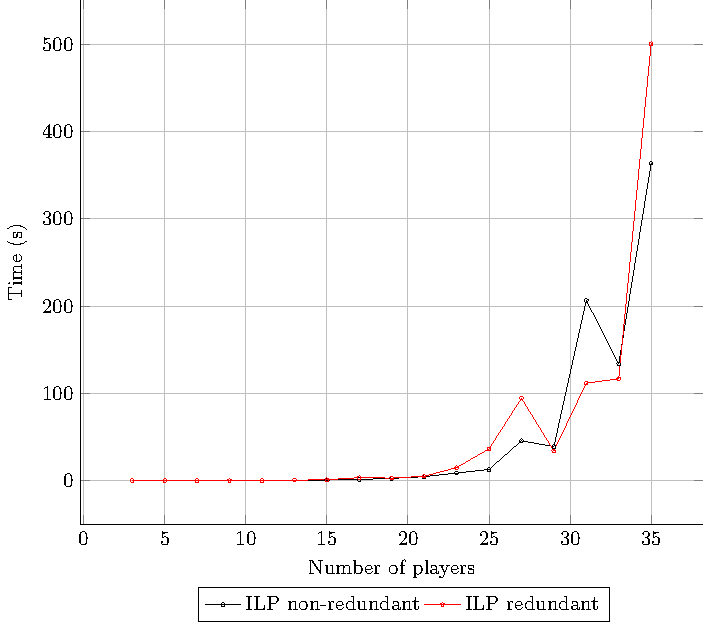
\includegraphics[width=\linewidth]{plots/time_per_instance.pdf}
    \caption{ILP runtime w.r.t the number of players}
    \label{figilp}
\end{figure}
\end{minipage}


\clearpage

\section{Meta-heuristics}
\textit{For the meta-heuristics, the pseudo-code of your constructive, local search and GRASP algorithms, including equations for describing the greedy cost function(s) and the RCL}

As a solution must exist no matter which player rests in a given day, we will focus on assigning a rest day for every player $p$. This information is enough for calculating our objective function, performing local search and GRASP. After all this, we will construct the pairings for the whole tournament.

\subsection{Constructive}

The greedy cost function is the points that a player $p$ assigns to resting on day $d$. As we want to maximize this, we will sort the available players in descending order and pick the one with highest value.

\begin{algorithm}
	\caption{Greedy algorithm} 
	\begin{algorithmic}[1]
	  \State Players $\leftarrow$ Set of Players
	  \State rests $\leftarrow$ \{\}
	    \For {day in 0..days}
	      \State playersToRest $\leftarrow$ filter Players(p) $|$ p.hasNotRested
	      \State sortedPlayers $\leftarrow$ sort playersToRest(p) by p.points[day] (DESC) 
	      \State select p $\in$ sortedPlayers[0]
	      \State rests[day]\ $\leftarrow$\ p
	    \EndFor
	\end{algorithmic} 
\end{algorithm}


\subsection{Local search}

In the local search phase we evaluate if swapping the players that rest in two given days increases our objective function\footnote{For simplicity, we initialize the best\_swap so that the local search doesn't change the solution if we found no improvement}.

\begin{algorithm}
	\caption{Local Search} 
	\begin{algorithmic}[1]
    \For {i in 0..days}
    \State best\_swap\_points $\leftarrow$ 0
    \State best\_swap $\leftarrow$ i
      \For {j in 0..days}
        \State change = EvaluateRestSwap(i,j)
        \If{change $>$ best\_swap\_points}
          \State best\_swap\_points $\leftarrow$ change
          \State best\_swap $\leftarrow$ j
        \EndIf
      \EndFor
      \State rests[i] $\leftrightarrow$ rests[best\_swap]
		\EndFor
	\end{algorithmic} 
\end{algorithm}

We can repeat this procedure iteratively until the local search provides no further improvement just by adding an outer loop.


\clearpage
\subsection{GRASP}

In the GRASP we randomize the selection of the player in descending order by points, according to a RCL calculated by $\alpha$.

\begin{algorithm}
	\caption{GRASP} 
	\begin{algorithmic}[1]
	  \State Players $\leftarrow$ Set of Players
	  \State rests $\leftarrow$ \{\}
	    \For {day in 0..days}]b
	      \State playersToRest $\leftarrow$ filter Players(p) $|$ p.hasNotRested
	      \State sortedPlayers $\leftarrow$ sort PlayersToRest(p) by p.points[day] (DESC) 
        \State $q_{max} \leftarrow $ sortedPlayers.first.points
        \State $q_{min} \leftarrow$ sortedPlayers.last.points
        \State $RCL_{max}$ $\leftarrow$ $\{p \in sortedPlayers\ |\ p.Points >= q_{max} - \alpha * (q_{max} - q_{min})\}$
	      \State select p $\in$ RCL at random
	      \State rests[day]\ $\leftarrow$\ p
	    \EndFor
	\end{algorithmic} 
\end{algorithm}

We must repeat this algorithm iteratively, having some stop conditions as a MAX\_ITER and a MAX\_ITER\_NOTIMPROVED. In this way, we put a maximum of iterations and a maximum of iterations without improve the objective function.


\section{Parameter tuning}

\section{Results}

\section{Reproducing the results}
%\todo[inline]{maybe setup a script to reproduce results or something...}

\begin{itemize}
    \item OPL source code
    \item Programs of the meta-heuristics
    \item Instance generator
    \item Instructions how to use every of them and how to reproduce results
\end{itemize}



\end{document}
